% fig:type_chart -- the values taken by the dimension function d(P) on
% projections, one number line per factor type.
% Included at 0.88\textwidth (~14.5 cm); drawn at roughly that natural width.
\documentclass[tikz,border=4pt]{standalone}
\usepackage{lmodern}
\usepackage{amsmath,amssymb}
\usepackage{xcolor}
\usepackage{tikz}
\usetikzlibrary{arrows.meta,calc}

\definecolor{ruleblue}{HTML}{2b6cb0}
\definecolor{rulegold}{HTML}{b7791f}
\definecolor{rulered}{HTML}{c0392b}

\begin{document}
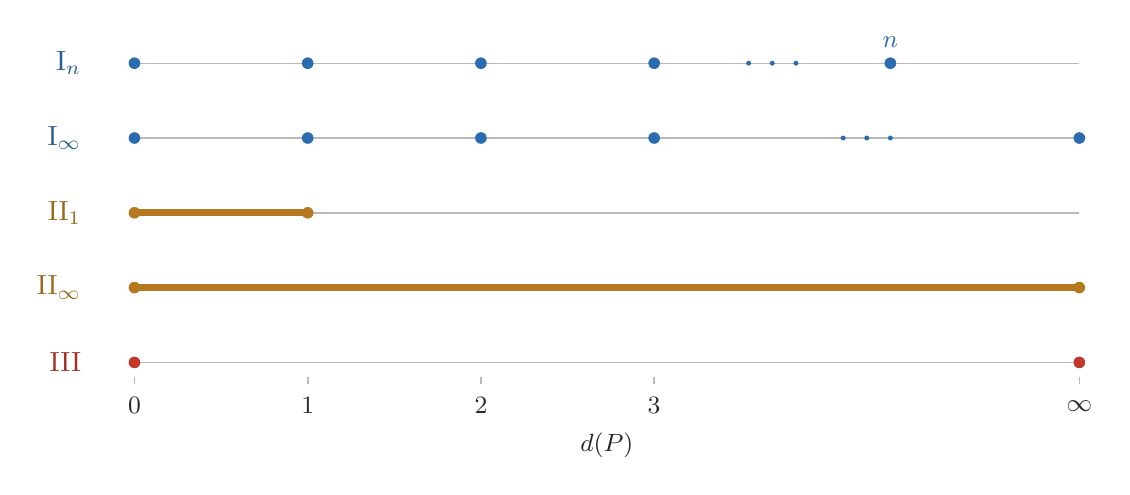
\begin{tikzpicture}[every node/.style={font=\small}, line width=0.6pt,
  dot/.style={circle, fill, inner sep=0pt, minimum size=4.2pt},
  axis/.style={gray!55, line width=0.5pt}]

% horizontal positions of 0, 1, 2, 3, n and infinity
\def\xone{2.2}\def\xtwo{4.4}\def\xthree{6.6}\def\xn{9.6}\def\xinf{12.0}
\def\dy{0.95}

% type-name column
\foreach \name/\k/\col in {{$\mathrm{I}_n$}/0/ruleblue, {$\mathrm{I}_\infty$}/1/ruleblue,
                           {$\mathrm{II}_1$}/2/rulegold, {$\mathrm{II}_\infty$}/3/rulegold,
                           {$\mathrm{III}$}/4/rulered}{
  \node[anchor=east, text=\col!85!black, font=\normalsize] at (-0.55,-\k*\dy) {\name};
  \draw[axis] (0,-\k*\dy) -- (\xinf,-\k*\dy);
}

% I_n : 0,1,2,3, ..., n
\begin{scope}[ruleblue, yshift=0cm]
  \foreach \x in {0,\xone,\xtwo,\xthree,\xn} \node[dot] at (\x,0) {};
  \foreach \t in {-0.3,0,0.3} \fill ({(\xthree+\xn)/2+\t},0) circle (0.9pt);
  \node[above=2pt] at (\xn,0) {$n$};
\end{scope}

% I_inf : 0,1,2,3, ..., infinity
\begin{scope}[ruleblue, yshift=-\dy cm]
  \foreach \x in {0,\xone,\xtwo,\xthree,\xinf} \node[dot] at (\x,0) {};
  \foreach \t in {-0.3,0,0.3} \fill ({(\xthree+\xinf)/2+\t},0) circle (0.9pt);
\end{scope}

% II_1 : the interval [0,1]
\begin{scope}[rulegold, yshift=-2*\dy cm]
  \draw[line width=2.4pt, line cap=round] (0,0) -- (\xone,0);
  \node[dot] at (0,0) {}; \node[dot] at (\xone,0) {};
\end{scope}

% II_inf : the interval [0,infinity]
\begin{scope}[rulegold, yshift=-3*\dy cm]
  \draw[line width=2.4pt, line cap=round] (0,0) -- (\xinf,0);
  \node[dot] at (0,0) {}; \node[dot] at (\xinf,0) {};
\end{scope}

% III : only 0 and infinity
\begin{scope}[rulered, yshift=-4*\dy cm]
  \node[dot] at (0,0) {}; \node[dot] at (\xinf,0) {};
\end{scope}

% common tick labels, below the last row
\def\yt{-4*\dy-0.55}
\foreach \x/\lab in {0/$0$, \xone/$1$, \xtwo/$2$, \xthree/$3$, \xinf/$\infty$}{
  \draw[gray!55] (\x,{-4*\dy-0.18}) -- (\x,{-4*\dy-0.28});
  \node[gray!30!black] at (\x,{\yt}) {\lab};
}
\node[gray!30!black] at ({\xinf/2},{\yt-0.5}) {$d(P)$};

\end{tikzpicture}
\end{document}
